\documentclass{article}\usepackage[]{graphicx}\usepackage[]{color}
%% maxwidth is the original width if it is less than linewidth
%% otherwise use linewidth (to make sure the graphics do not exceed the margin)
\makeatletter
\def\maxwidth{ %
  \ifdim\Gin@nat@width>\linewidth
    \linewidth
  \else
    \Gin@nat@width
  \fi
}
\makeatother

\definecolor{fgcolor}{rgb}{0.345, 0.345, 0.345}
\newcommand{\hlnum}[1]{\textcolor[rgb]{0.686,0.059,0.569}{#1}}%
\newcommand{\hlstr}[1]{\textcolor[rgb]{0.192,0.494,0.8}{#1}}%
\newcommand{\hlcom}[1]{\textcolor[rgb]{0.678,0.584,0.686}{\textit{#1}}}%
\newcommand{\hlopt}[1]{\textcolor[rgb]{0,0,0}{#1}}%
\newcommand{\hlstd}[1]{\textcolor[rgb]{0.345,0.345,0.345}{#1}}%
\newcommand{\hlkwa}[1]{\textcolor[rgb]{0.161,0.373,0.58}{\textbf{#1}}}%
\newcommand{\hlkwb}[1]{\textcolor[rgb]{0.69,0.353,0.396}{#1}}%
\newcommand{\hlkwc}[1]{\textcolor[rgb]{0.333,0.667,0.333}{#1}}%
\newcommand{\hlkwd}[1]{\textcolor[rgb]{0.737,0.353,0.396}{\textbf{#1}}}%
\let\hlipl\hlkwb

\usepackage{framed}
\makeatletter
\newenvironment{kframe}{%
 \def\at@end@of@kframe{}%
 \ifinner\ifhmode%
  \def\at@end@of@kframe{\end{minipage}}%
  \begin{minipage}{\columnwidth}%
 \fi\fi%
 \def\FrameCommand##1{\hskip\@totalleftmargin \hskip-\fboxsep
 \colorbox{shadecolor}{##1}\hskip-\fboxsep
     % There is no \\@totalrightmargin, so:
     \hskip-\linewidth \hskip-\@totalleftmargin \hskip\columnwidth}%
 \MakeFramed {\advance\hsize-\width
   \@totalleftmargin\z@ \linewidth\hsize
   \@setminipage}}%
 {\par\unskip\endMakeFramed%
 \at@end@of@kframe}
\makeatother

\definecolor{shadecolor}{rgb}{.97, .97, .97}
\definecolor{messagecolor}{rgb}{0, 0, 0}
\definecolor{warningcolor}{rgb}{1, 0, 1}
\definecolor{errorcolor}{rgb}{1, 0, 0}
\newenvironment{knitrout}{}{} % an empty environment to be redefined in TeX

\usepackage{alltt}
\usepackage[utf8]{inputenc}
\usepackage{hyperref}
\hypersetup{
  linktocpage,
  colorlinks=true, 
  linkcolor=blue,
  citecolor=blue,
  filecolor=blue,
  urlcolor=blue,
}
\IfFileExists{upquote.sty}{\usepackage{upquote}}{}
\begin{document}

\title{Metilació i Acetilació a 10G i 1.2B}
\author{Alfred Cortés i Lucas Michel Todó}
\maketitle
\tableofcontents
\clearpage
\section{Introducció}
Les dades representades en aquest set de gràfiques representen l'acetilació i meilació de de les mostres 10G i 1.2B del nostre estudi de Chip-Seq. El genoma sencer de les dues mostres s'ha partit en fragments de 200bp que s'on els que conformen la base de les dades representades. Cada fragment de 200bp porta associada informació respecte el gen a què correspon, l'estat d'acetilació i metilació i si correspon a una zona 3',5' o ORF. 
\clearpage
\begin{knitrout}
\definecolor{shadecolor}{rgb}{0.969, 0.969, 0.969}\color{fgcolor}\begin{kframe}


{\ttfamily\noindent\bfseries\color{errorcolor}{\#\# Error in library(pscl): there is no package called 'pscl'}}

{\ttfamily\noindent\bfseries\color{errorcolor}{\#\# Error in library(XLConnect): there is no package called 'XLConnect'}}\end{kframe}
\end{knitrout}





\begin{knitrout}
\definecolor{shadecolor}{rgb}{0.969, 0.969, 0.969}\color{fgcolor}\begin{kframe}


{\ttfamily\noindent\bfseries\color{errorcolor}{\#\# Error in readWorksheetFromFile("{}/home/lucas/ISGlobal/Chip\_Seq/Transcripció\_CSV/3D7\_Variantome\_AllData\_withGam.xls"{}, : could not find function "{}readWorksheetFromFile"{}}}

{\ttfamily\noindent\bfseries\color{errorcolor}{\#\# Error in eval(expr, envir, enclos): object 'trans\_df' not found}}

{\ttfamily\noindent\bfseries\color{errorcolor}{\#\# Error in eval(expr, envir, enclos): object 'trans\_df' not found}}

{\ttfamily\noindent\bfseries\color{errorcolor}{\#\# Error in eval(expr, envir, enclos): object 'trans\_df' not found}}

{\ttfamily\noindent\bfseries\color{errorcolor}{\#\# Error in ref\$ID \%in\% noexprs: object 'noexprs' not found}}

{\ttfamily\noindent\bfseries\color{errorcolor}{\#\# Error in eval(expr, envir, enclos): object 'noexprs\_df' not found}}\end{kframe}
\end{knitrout}

\section{Histogrames}
En primer lloc hem representat la distribució dels valors d'acetilació i de metilació als fragments (de 10G). (Archiu "Coverage\_10G\_200bp.csv", 116656 fragments corresponents al genoma sencer. Coverage directament del "bam" nomralitzat per nombre de reads.)
\subsection{log(Ac) All}
\begin{knitrout}
\definecolor{shadecolor}{rgb}{0.969, 0.969, 0.969}\color{fgcolor}

{\centering 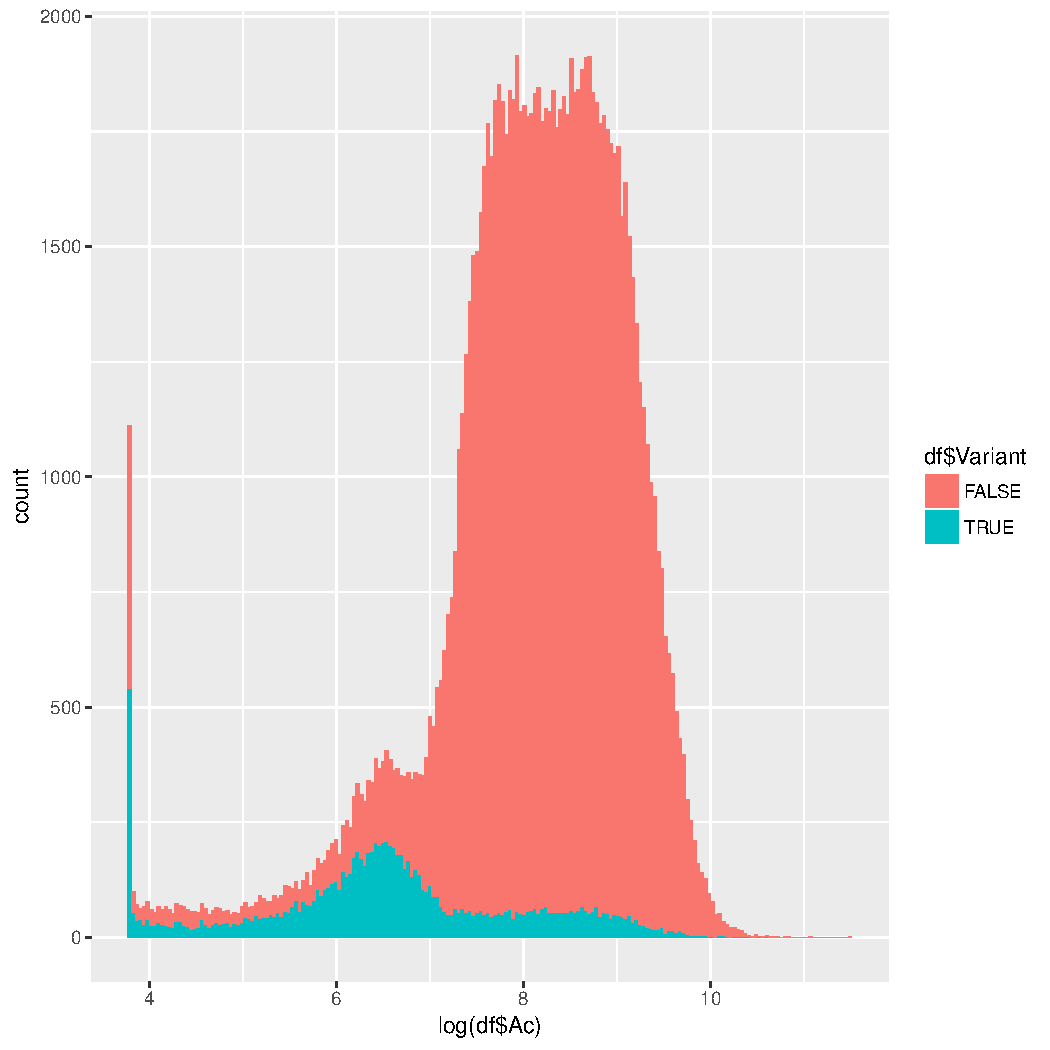
\includegraphics[width=1\linewidth]{figure/minimal-dens_all-1} 

}



\end{knitrout}
\clearpage
\subsection{log(Ac) 5'}
\begin{knitrout}
\definecolor{shadecolor}{rgb}{0.969, 0.969, 0.969}\color{fgcolor}

{\centering 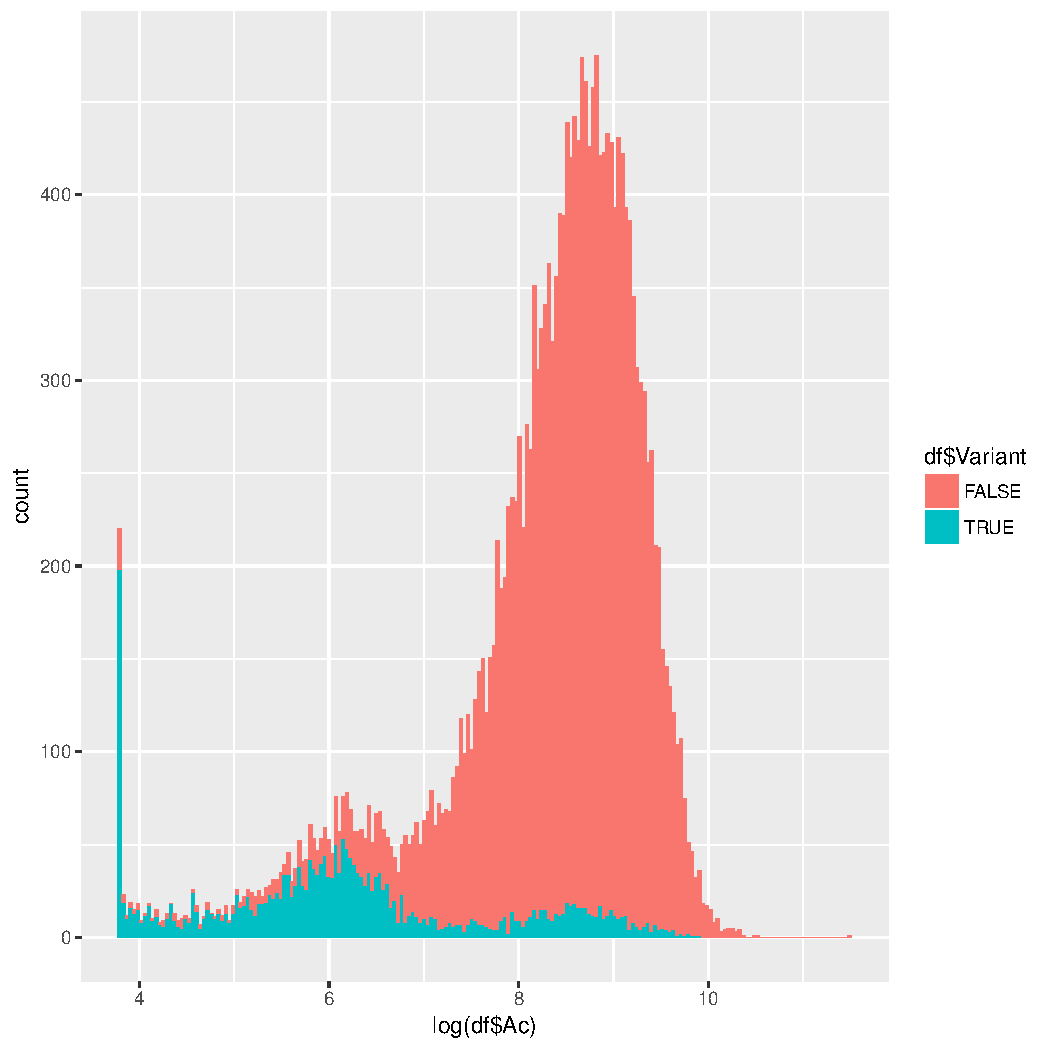
\includegraphics[width=1\linewidth]{figure/minimal-dens_5-1} 

}



\end{knitrout}
\clearpage
\subsection{log(Ac) 3'}
\begin{knitrout}
\definecolor{shadecolor}{rgb}{0.969, 0.969, 0.969}\color{fgcolor}

{\centering 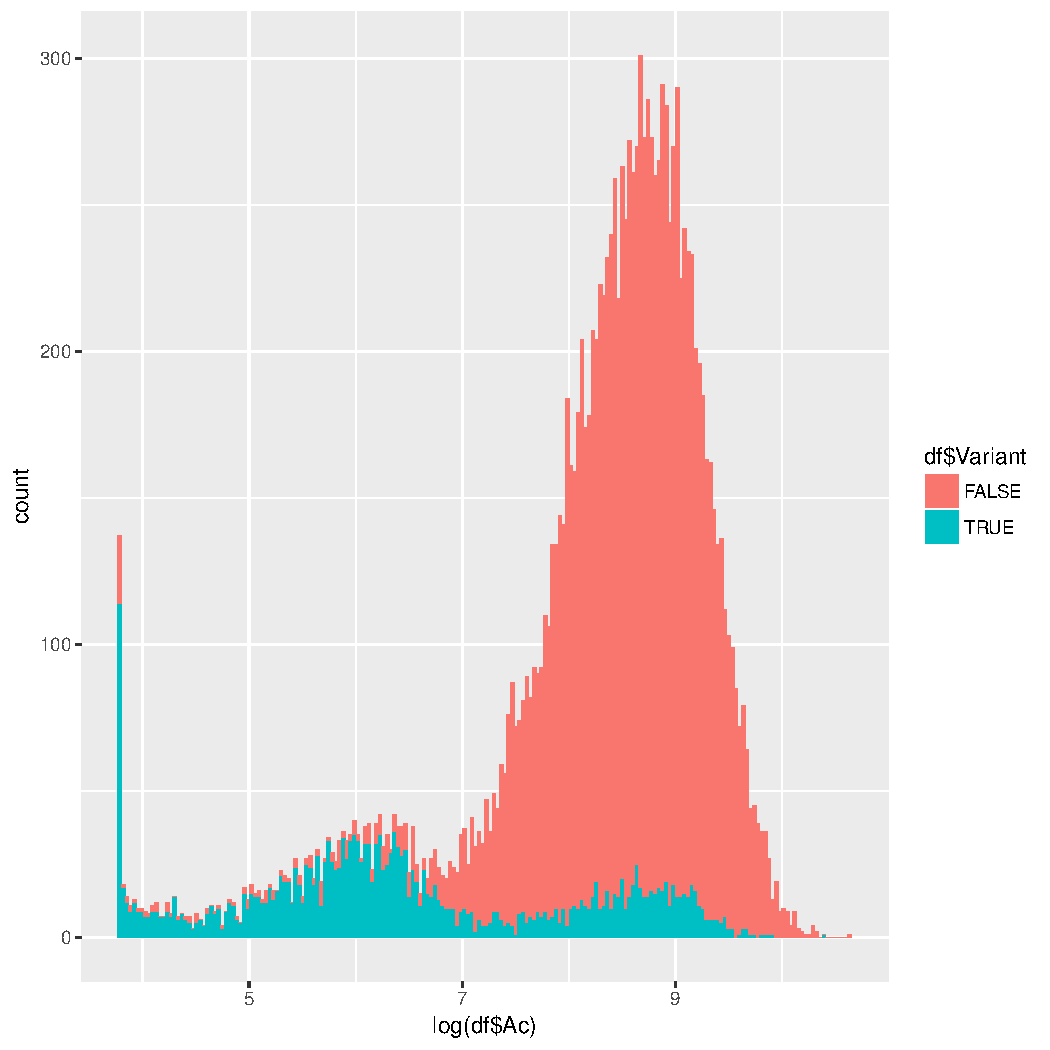
\includegraphics[width=1\linewidth]{figure/minimal-dens_3-1} 

}



\end{knitrout}
\clearpage
\subsection{log(Ac) ORF}
\begin{knitrout}
\definecolor{shadecolor}{rgb}{0.969, 0.969, 0.969}\color{fgcolor}

{\centering 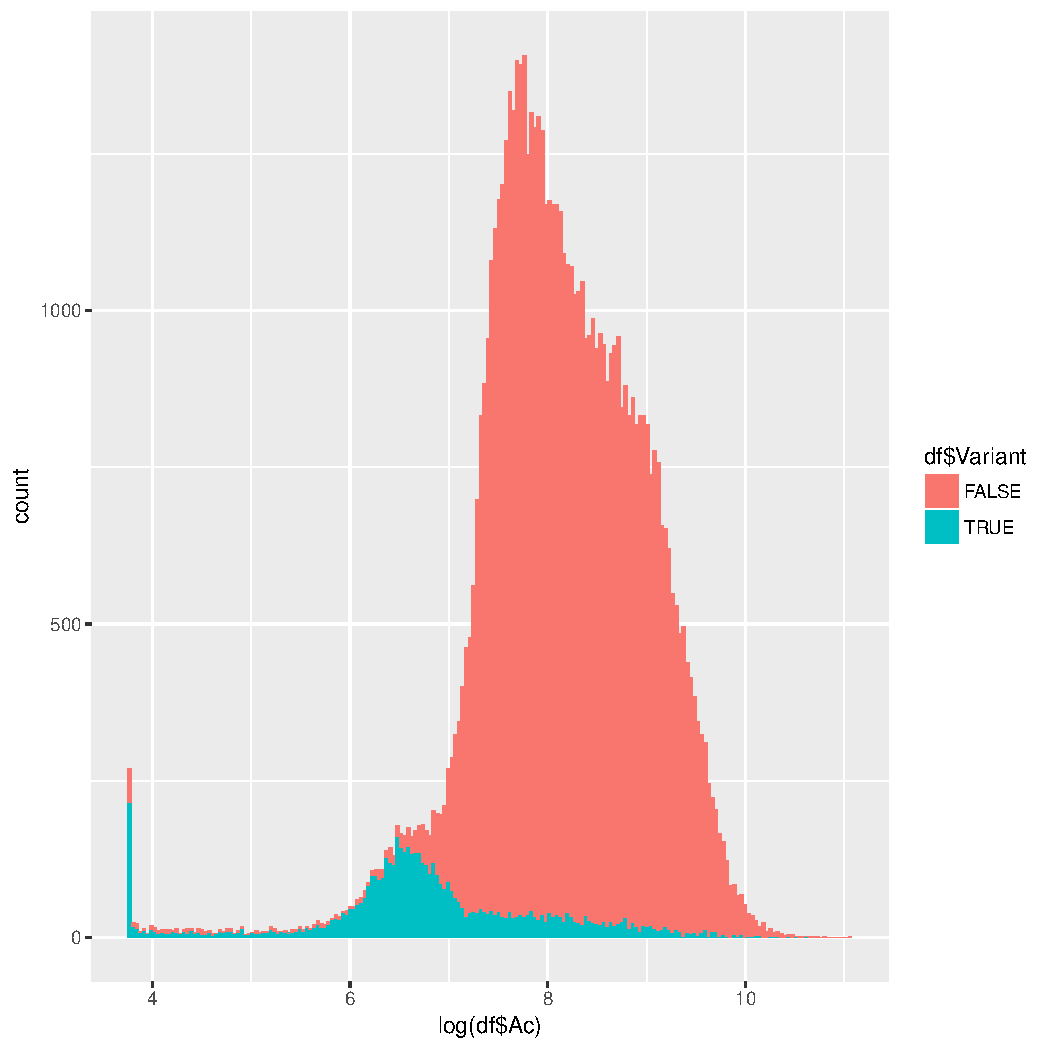
\includegraphics[width=1\linewidth]{figure/minimal-dens_ORF-1} 

}



\end{knitrout}
\clearpage
\subsection{log(Met) All}
\begin{knitrout}
\definecolor{shadecolor}{rgb}{0.969, 0.969, 0.969}\color{fgcolor}

{\centering 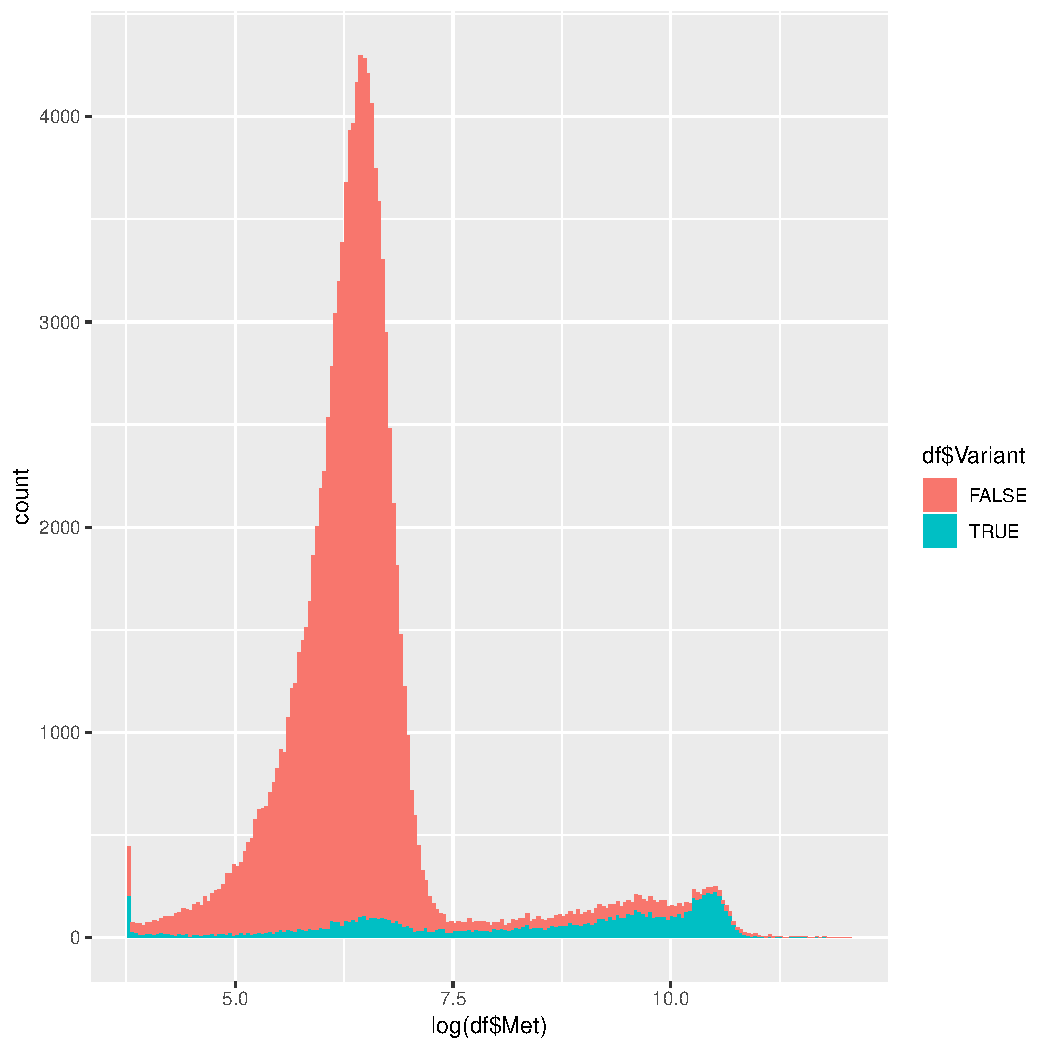
\includegraphics[width=1\linewidth]{figure/minimal-dens_all_met-1} 

}



\end{knitrout}
\clearpage
\subsection{log(Met) 5'}
\begin{knitrout}
\definecolor{shadecolor}{rgb}{0.969, 0.969, 0.969}\color{fgcolor}

{\centering 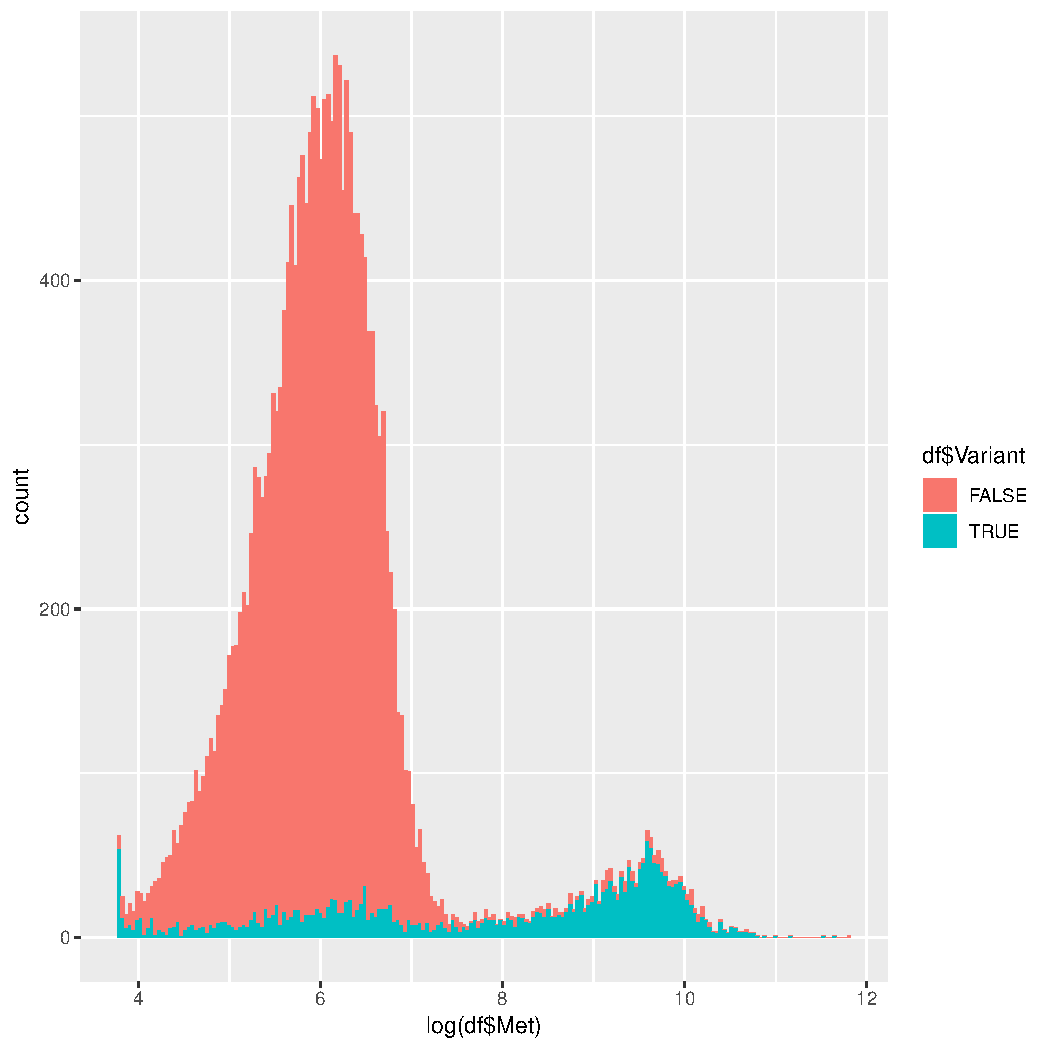
\includegraphics[width=1\linewidth]{figure/minimal-dens_5_met-1} 

}



\end{knitrout}
\clearpage
\subsection{log(Met) ORF}
\begin{knitrout}
\definecolor{shadecolor}{rgb}{0.969, 0.969, 0.969}\color{fgcolor}

{\centering 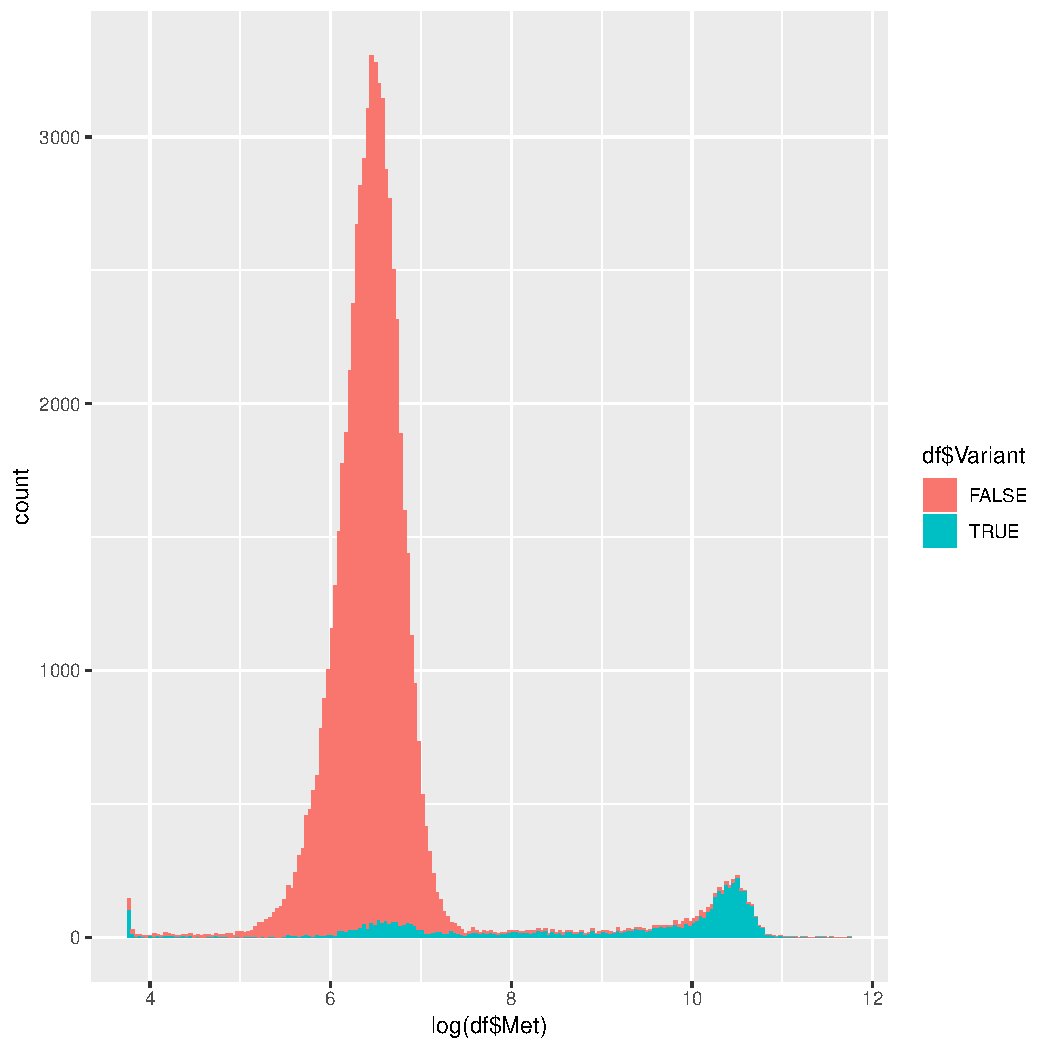
\includegraphics[width=1\linewidth]{figure/minimal-dens_ORF_met-1} 

}



\end{knitrout}
\clearpage
\subsection{log(Ac) 3'}
\begin{knitrout}
\definecolor{shadecolor}{rgb}{0.969, 0.969, 0.969}\color{fgcolor}

{\centering 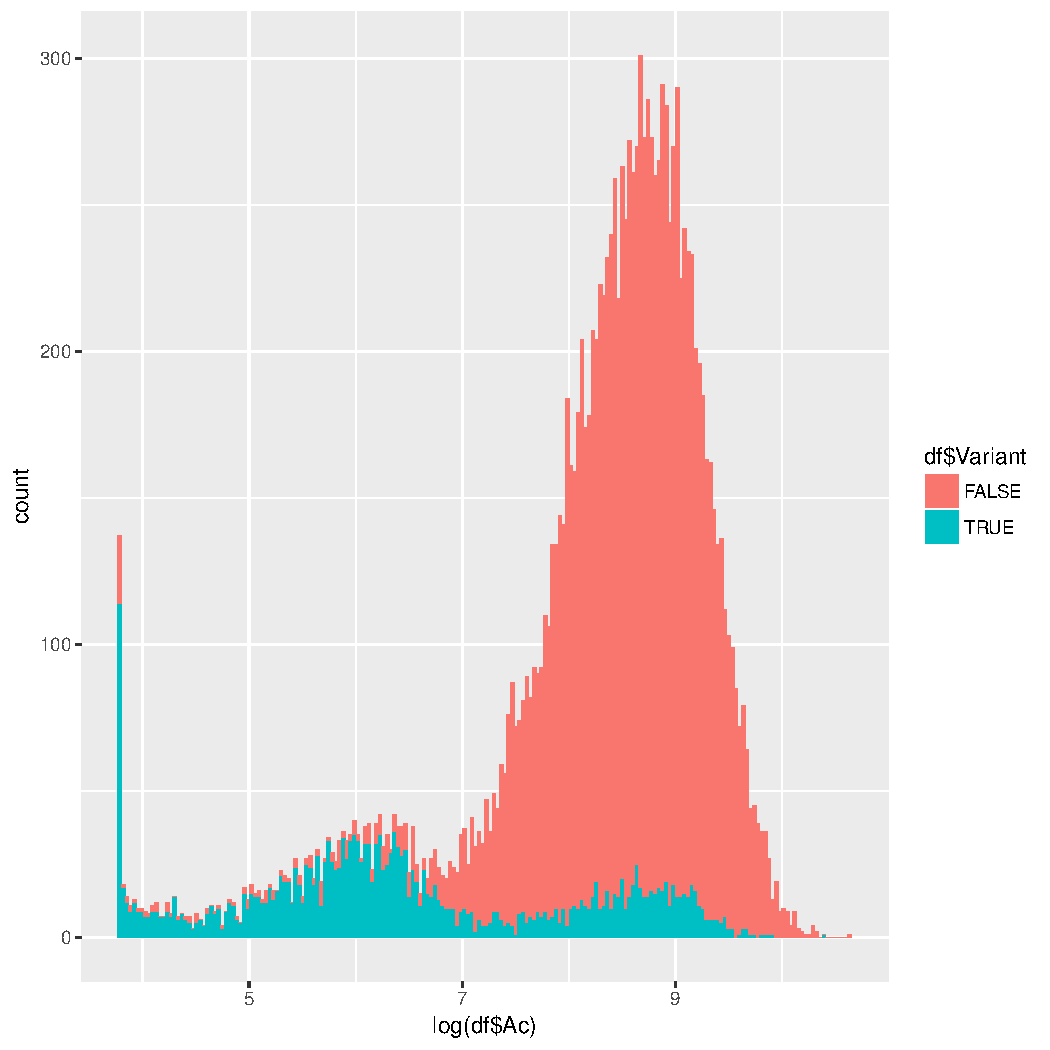
\includegraphics[width=1\linewidth]{figure/minimal-dens_3_met-1} 

}



\end{knitrout}
\clearpage

\section{Acetilació vs Metilació}
A continuació hem volgut dilucidar si la combinació de l'estat de metilació i acetilació dels fragments ens permet diferenciar entre gens variants/no-variants i entre els gens variants actius/incatius.

Hem classificat els gens com a variants utilitzant una llista obtiniguda en un estudi anterior. (La llista de gens variants es troba a "Gens\_variants\_extended.txt", 514 gens. Aquesta informació s'ha expandit a tots els fragments que formen part d'aquests gens, 5' i 3' inclosos.)
\clearpage
\subsection{Transcripció i Metilació}
Per a poder classificar els gens com a variants actius/inactius peimer hem mirat la distribució de les dades de transcripció i les de metilació. (amb l'idea de trobar llindars per a expressat/no expressat, metilat/no metilat).
\begin{knitrout}
\definecolor{shadecolor}{rgb}{0.969, 0.969, 0.969}\color{fgcolor}\begin{kframe}


{\ttfamily\noindent\bfseries\color{errorcolor}{\#\# Error in ggplot(trans\_df, aes(log(trans\_df\$Aver.2Higher10G.))): object 'trans\_df' not found}}\end{kframe}
\end{knitrout}
\clearpage
\begin{knitrout}
\definecolor{shadecolor}{rgb}{0.969, 0.969, 0.969}\color{fgcolor}

{\centering 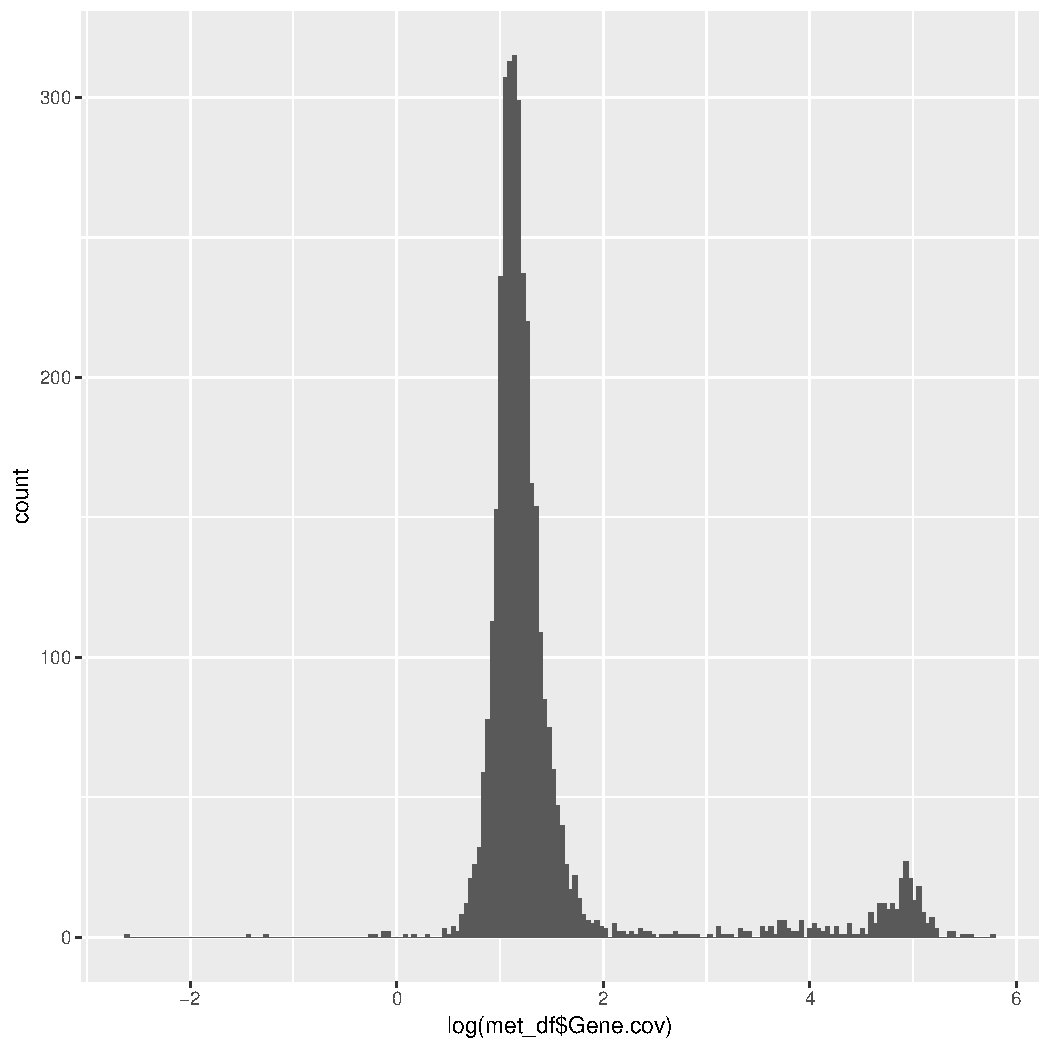
\includegraphics[width=1\linewidth]{figure/minimal-met_histo-1} 

}



\end{knitrout}
\clearpage
\subsection{Classificació segons Metilació}
En un primer intent de diferenciar variants actius d'inactius hem creat el paremetre "silenced" que hem considerat "TRUE" si el valor de metilació del fragment està per sobre d'un llindar ($>$3). (Els valors de metilació utilitzats corresponen a l'ORF de cada gen i s'han expandit a tots els fragments que en formen part.)
\begin{knitrout}
\definecolor{shadecolor}{rgb}{0.969, 0.969, 0.969}\color{fgcolor}\begin{kframe}
\begin{verbatim}
## 
##          Regular   Variant-Active Variant-Silenced 
##           105873             5317             5467
\end{verbatim}
\end{kframe}

{\centering 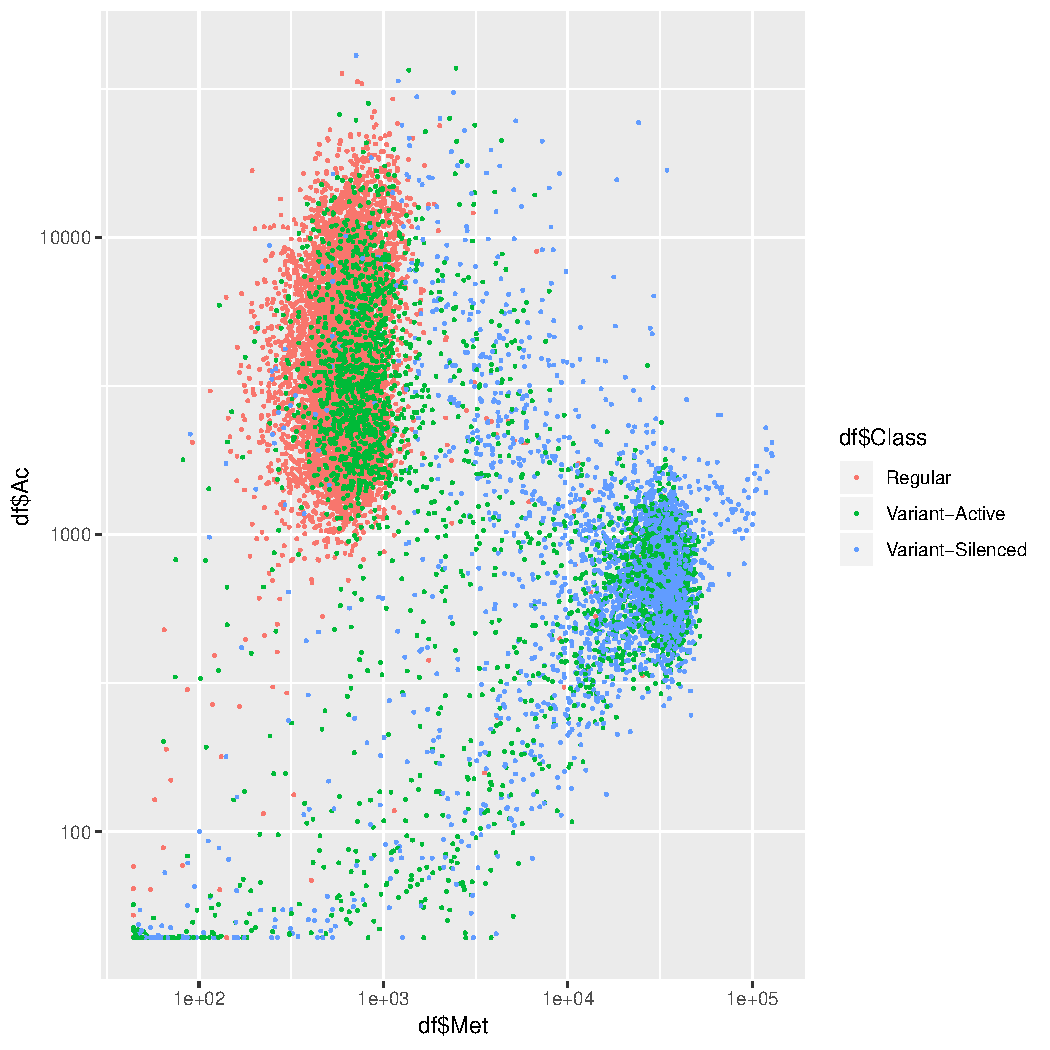
\includegraphics[width=1\linewidth]{figure/minimal-ac_met_log_status-1} 

}



\end{knitrout}
\clearpage
\subsection{Classificació segons Metilació i estat Transcripcional}
En un segon intent hem afegit la variable "noexprs" que hem considerat "TRUE" quan el valor d'expressió d'un fragment està per sota d'un llindar ($<$4)(Igual que en el cas anterior el valor de transcripció correspon a un gen i s'ha expandit a tots els fragments que en formen part.)(Dades de trascripció a l'arxiu "3D7\_Variantome\_AllData\_withGam.xls" fulla 1 columnes 1 i 26).
\begin{knitrout}
\definecolor{shadecolor}{rgb}{0.969, 0.969, 0.969}\color{fgcolor}

{\centering 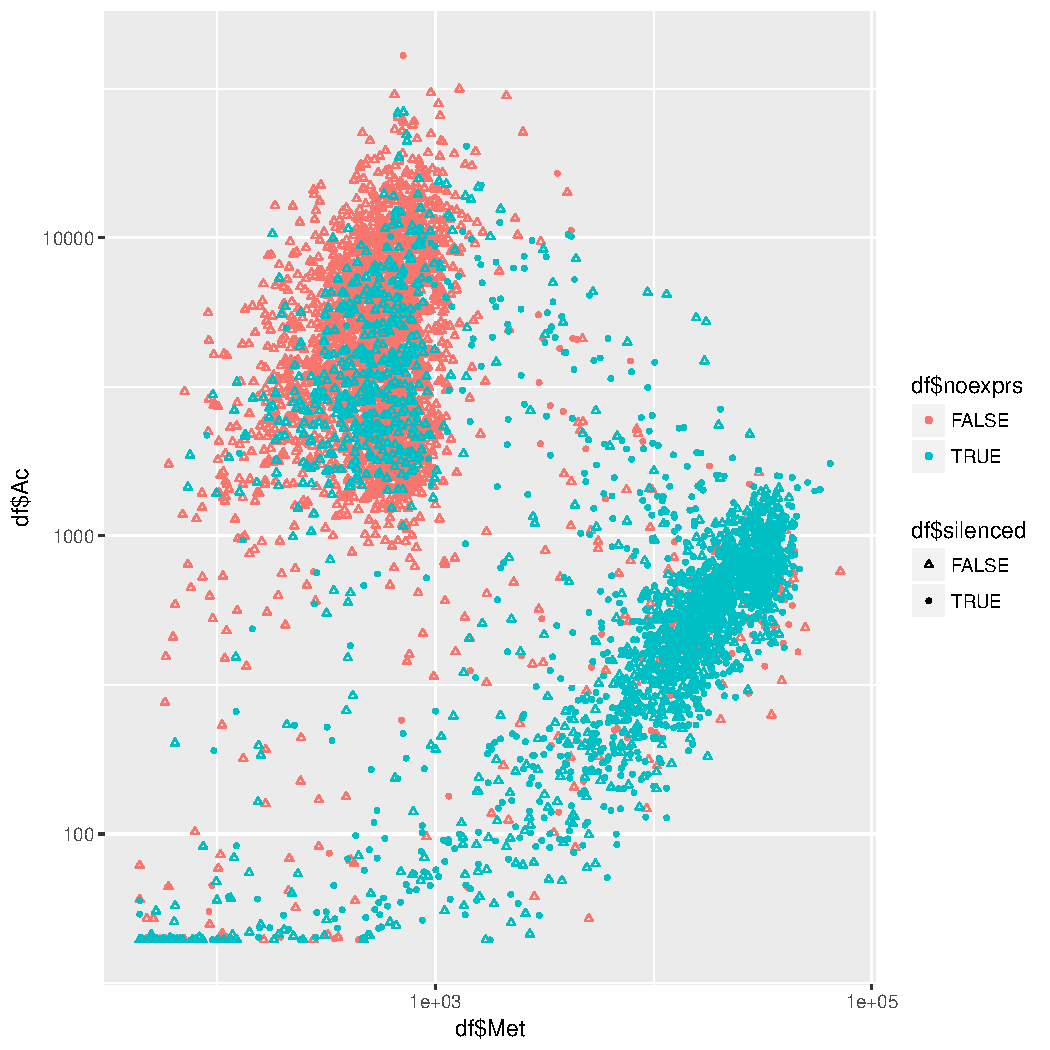
\includegraphics[width=1\linewidth]{figure/minimal-ac_met_log-1} 

}



\end{knitrout}
\clearpage
\subsection{Gens diferencials}
Finalment, vist que els anterior mètodes no enc classificaven satisfactòriament els gens com a variants actius o inactius, hem decidit centrar-nos en aquells gens que s'expressen diferencialment entre 10G i 1.2B. 
Els gens variants que estàn sobreexpressats en una soca respecte una altra els hem classificat com a actius i viceversa.
Al fons del gràfic hem afegit la resta de gens (tots aquells que no tenen una expressió diferencial.)
El que hi ha representat al gràfic són fragments de 200bp (tota la informació respectiva a gens s'ha traslladat als fragments que els representen). (Gens diferencials i nivells d'expressió a "Trans2.csv", 30 gens a la llista dels quals només usem els 20 amb majors diferències d'expressió.)
\clearpage
\subsubsection{Gràfic de Gens diferencials: ORF}
\begin{knitrout}
\definecolor{shadecolor}{rgb}{0.969, 0.969, 0.969}\color{fgcolor}

{\centering 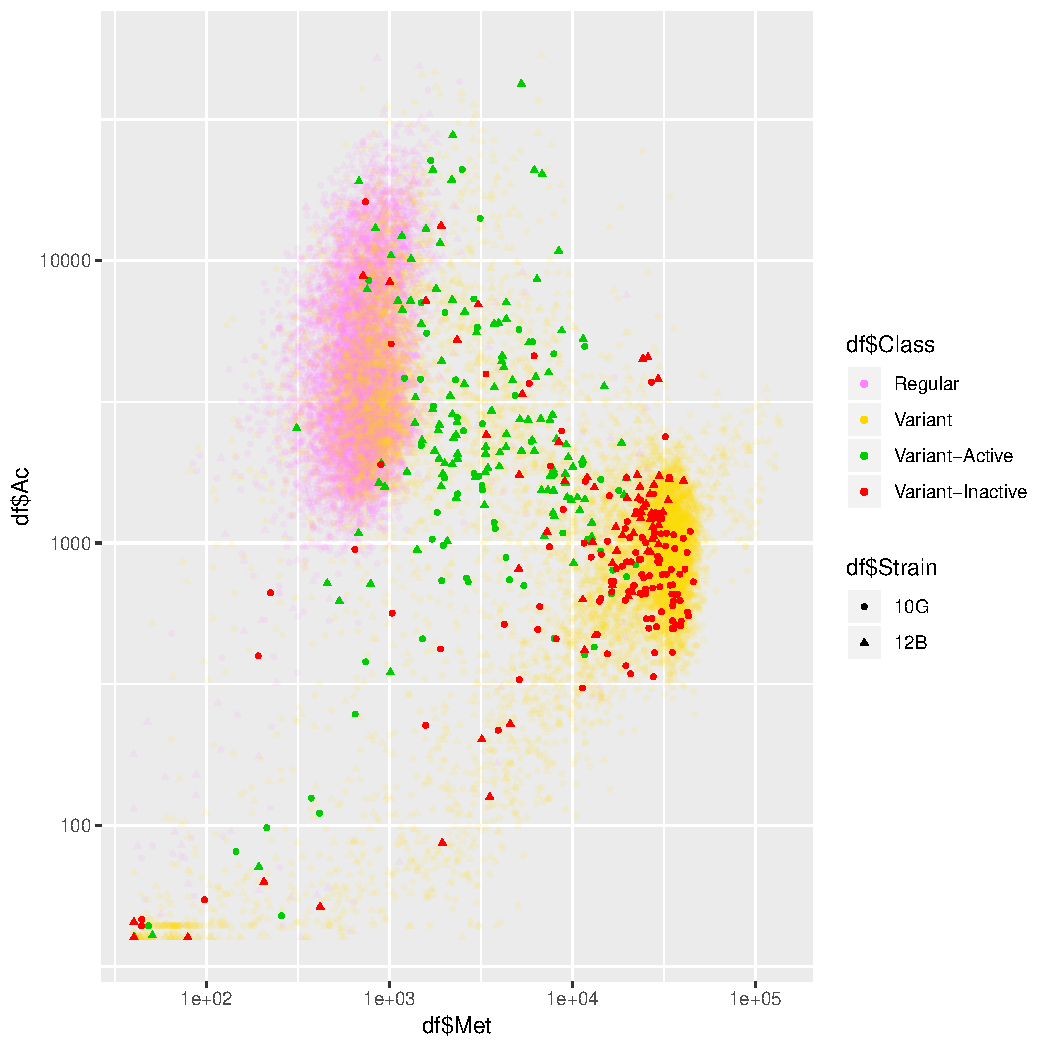
\includegraphics[width=1\linewidth]{figure/minimal-ac_met_log_status_10G_12B_ORF-1} 

}



\end{knitrout}
\clearpage
\subsubsection{Gràfic de Gens diferencials: 5'}
\begin{knitrout}
\definecolor{shadecolor}{rgb}{0.969, 0.969, 0.969}\color{fgcolor}

{\centering 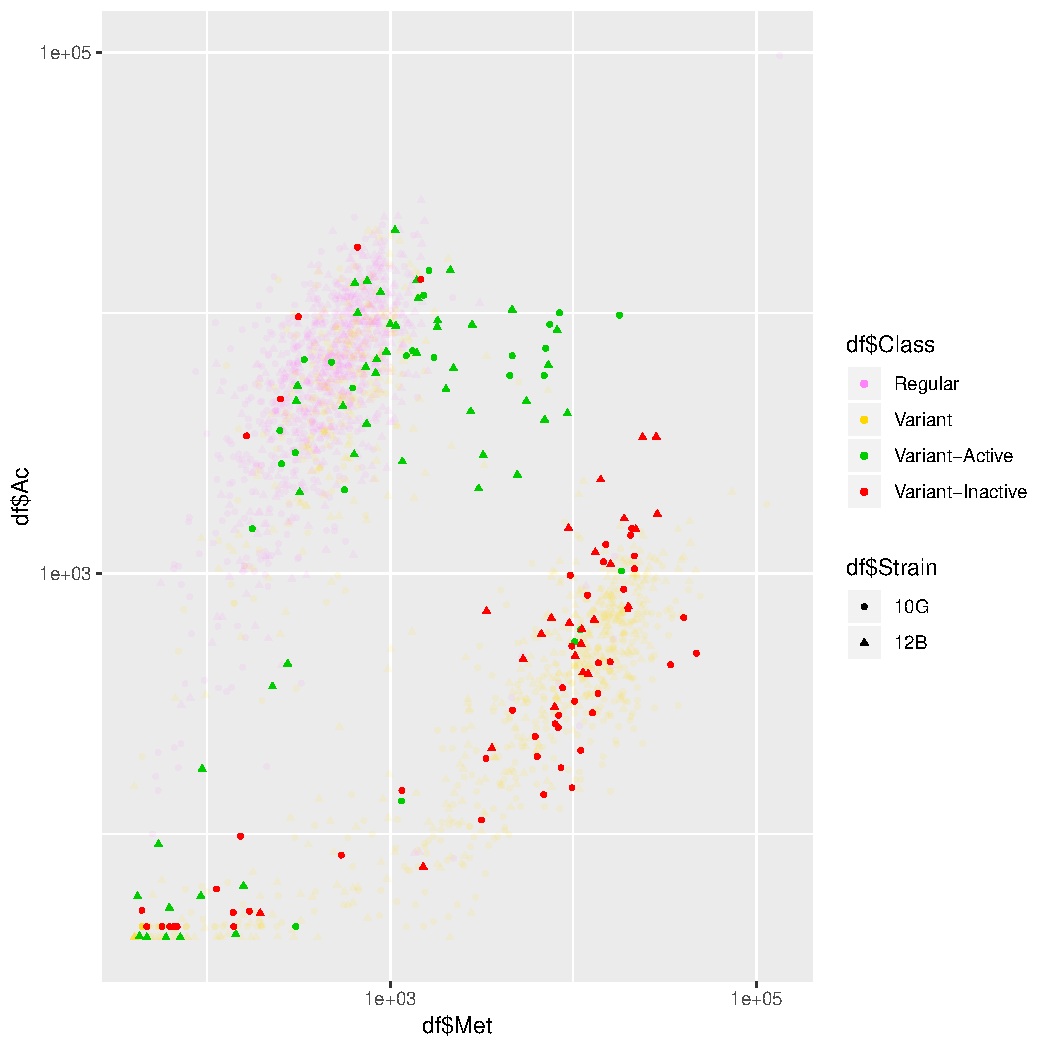
\includegraphics[width=1\linewidth]{figure/minimal-ac_met_log_status_10G_12B_5-1} 

}



\end{knitrout}
\clearpage
\subsubsection{Gràfic de Gens diferencials: 3'}
\begin{knitrout}
\definecolor{shadecolor}{rgb}{0.969, 0.969, 0.969}\color{fgcolor}

{\centering 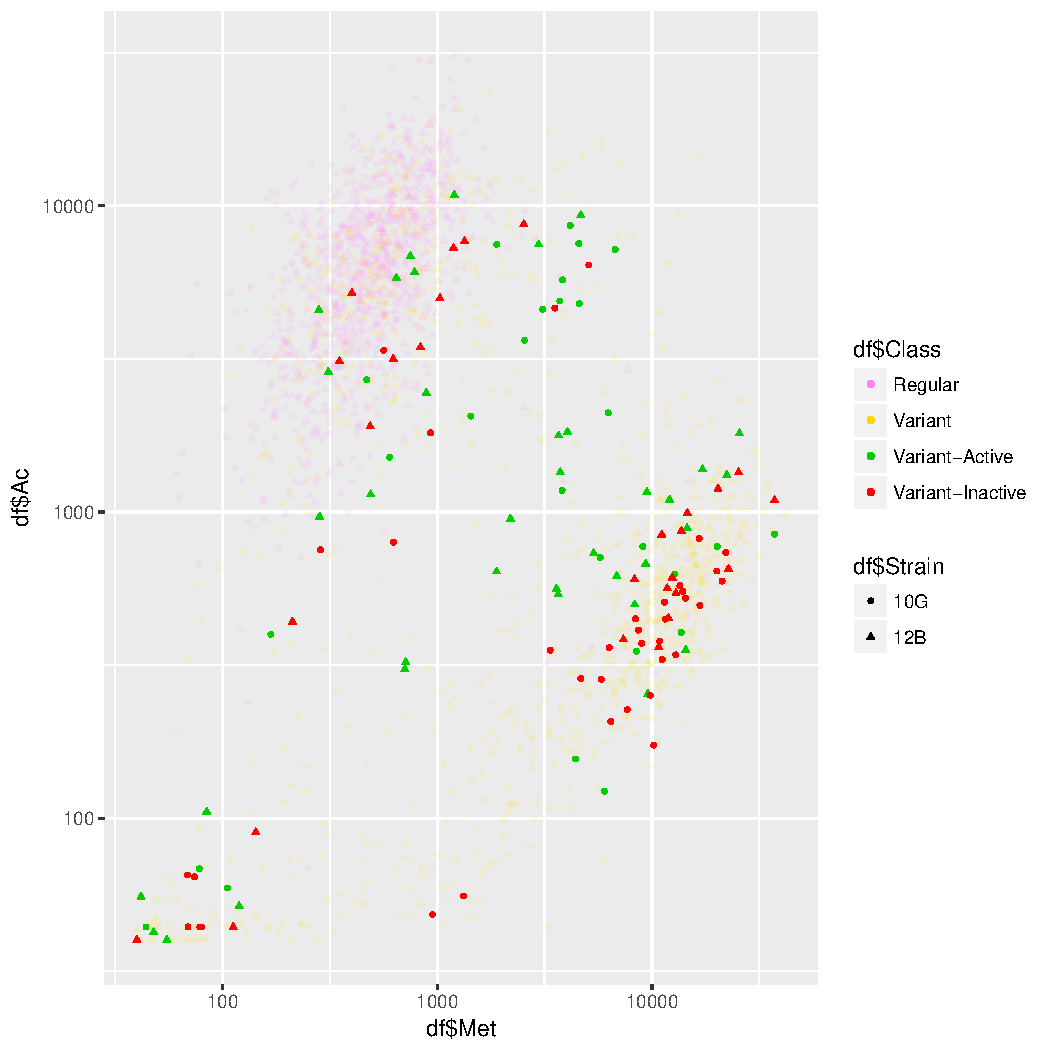
\includegraphics[width=1\linewidth]{figure/minimal-ac_met_log_status_10G_12B_3-1} 

}



\end{knitrout}
\clearpage
\subsubsection{Gràfic de Gens diferencials: Només Var i Rifin}
\begin{knitrout}
\definecolor{shadecolor}{rgb}{0.969, 0.969, 0.969}\color{fgcolor}

{\centering 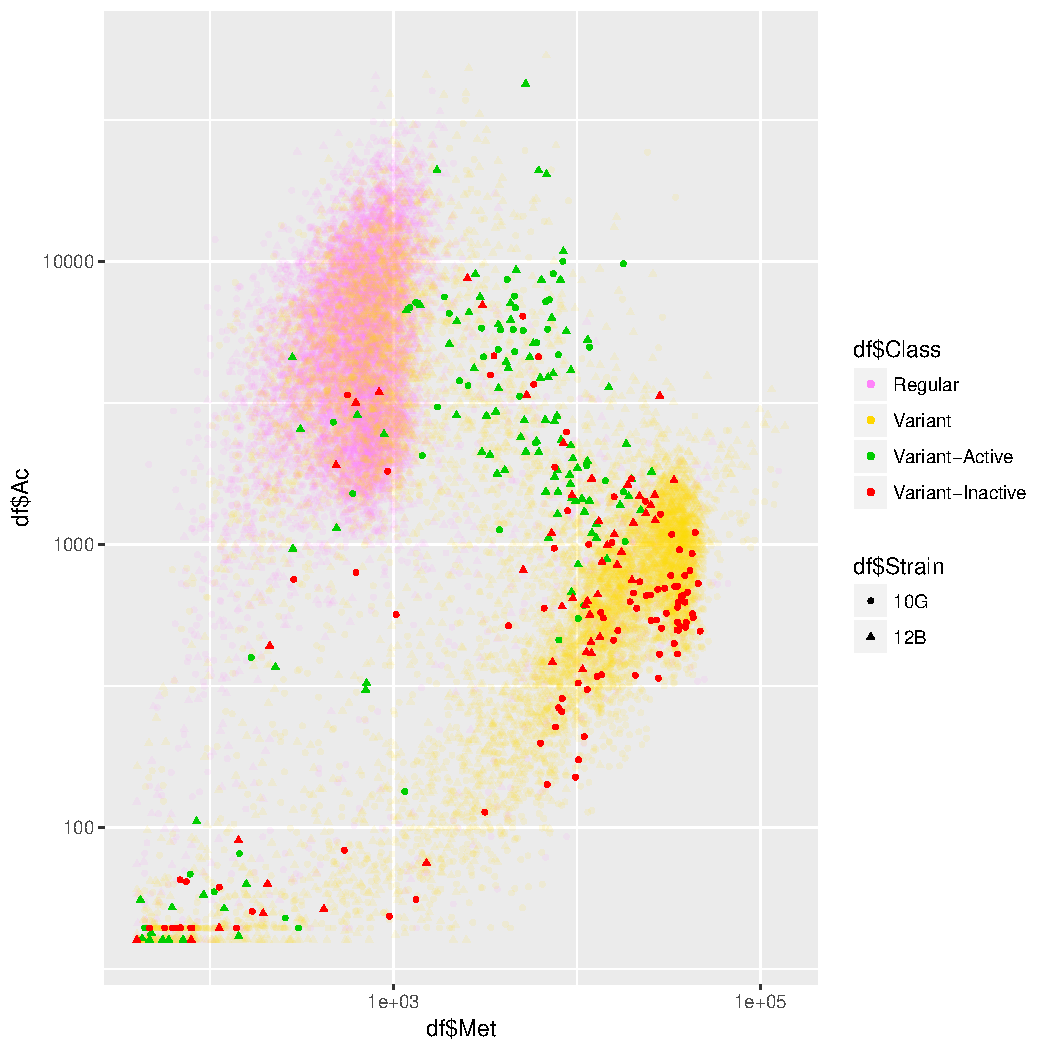
\includegraphics[width=1\linewidth]{figure/minimal-ac_met_log_status_10G_12B_varifin-1} 

}



\end{knitrout}
\clearpage
\subsubsection{Gràfic de Gens diferencials: Excepte Var i Rifin}
\begin{knitrout}
\definecolor{shadecolor}{rgb}{0.969, 0.969, 0.969}\color{fgcolor}

{\centering 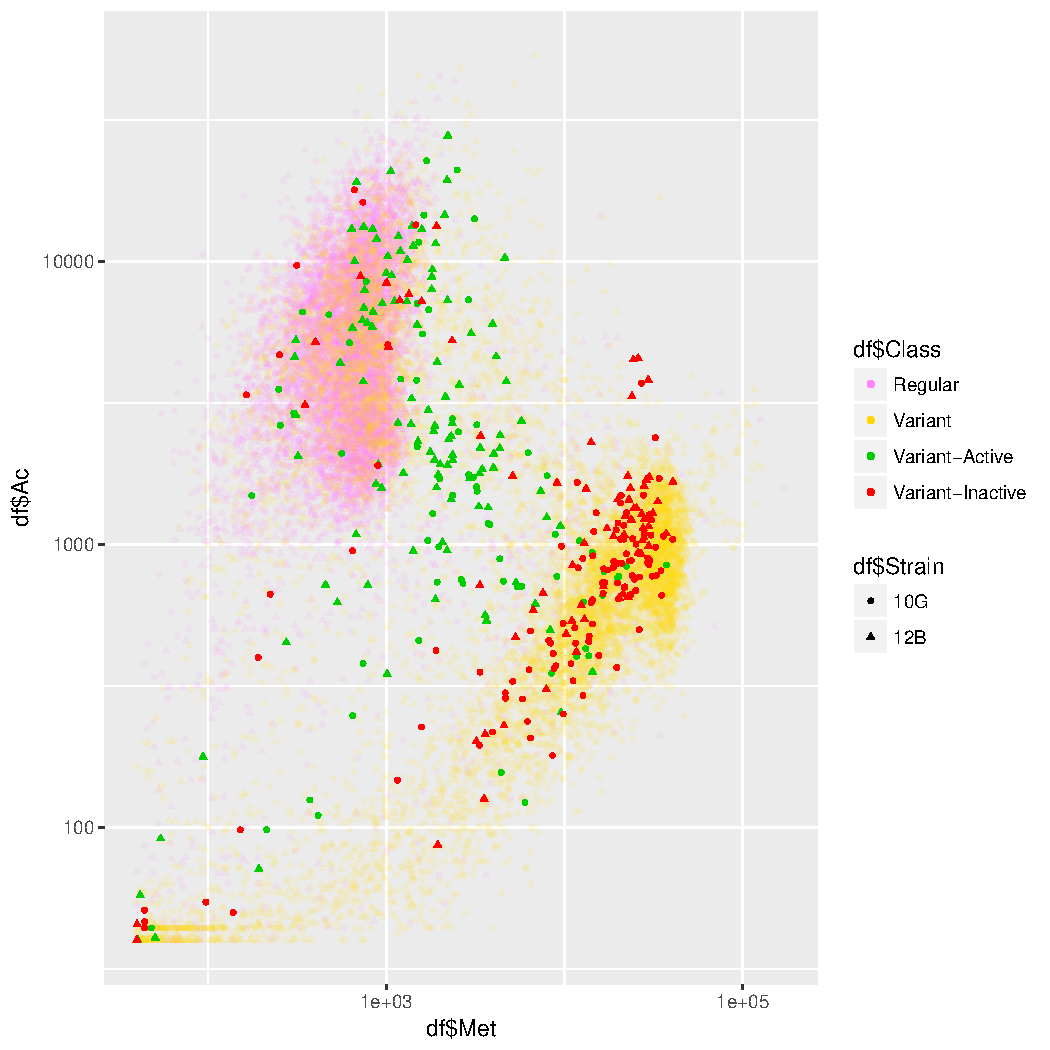
\includegraphics[width=1\linewidth]{figure/minimal-ac_met_log_status_10G_12B_novarifin-1} 

}



\end{knitrout}
\clearpage


\section{Model}
Finalment hem volgut comprovar si amb les dades de metilació i acetilació podiem crear un model basat en regressió logística que fós capaç de classificar correctament gens variants i no variants.
\begin{knitrout}
\definecolor{shadecolor}{rgb}{0.969, 0.969, 0.969}\color{fgcolor}\begin{kframe}
\begin{verbatim}
## 
##  FALSE   TRUE 
## 105873  10784
## Analysis of Deviance Table
## 
## Model 1: Variant ~ Ac + Met + Type + Start + Stop + silenced + noexprs
## Model 2: Variant ~ Ac + Met + Type + Start + Stop
##   Resid. Df Resid. Dev Df Deviance  Pr(>Chi)    
## 1      8478     5697.8                          
## 2      8479     6339.3 -1  -641.59 < 2.2e-16 ***
## ---
## Signif. codes:  0 '***' 0.001 '**' 0.01 '*' 0.05 '.' 0.1 ' ' 1
## 
## Call:
## glm(formula = Variant ~ Ac + Met + Type + Start + Stop + silenced + 
##     noexprs, family = binomial(link = "logit"), data = train_df)
## 
## Deviance Residuals: 
##     Min       1Q   Median       3Q      Max  
## -7.5153  -0.7720   0.0073   0.1886   3.0433  
## 
## Coefficients: (2 not defined because of singularities)
##                Estimate Std. Error z value Pr(>|z|)    
## (Intercept)   8.063e-01  9.816e-02   8.214  < 2e-16 ***
## Ac           -1.297e-04  9.454e-06 -13.720  < 2e-16 ***
## Met           3.064e-04  2.234e-05  13.715  < 2e-16 ***
## Type5prima   -3.511e-01  9.901e-02  -3.546 0.000391 ***
## TypeORF      -1.102e+00  8.637e-02 -12.758  < 2e-16 ***
## Typeother    -3.843e+01  1.200e+03  -0.032 0.974462    
## Start        -2.501e-07  4.152e-08  -6.025 1.69e-09 ***
## Stop                 NA         NA      NA       NA    
## silencedTRUE  4.148e+00  2.997e-01  13.840  < 2e-16 ***
## noexprsTRUE          NA         NA      NA       NA    
## ---
## Signif. codes:  0 '***' 0.001 '**' 0.01 '*' 0.05 '.' 0.1 ' ' 1
## 
## (Dispersion parameter for binomial family taken to be 1)
## 
##     Null deviance: 11150.5  on 8485  degrees of freedom
## Residual deviance:  5697.8  on 8478  degrees of freedom
## AIC: 5713.8
## 
## Number of Fisher Scoring iterations: 20
##        
##         FALSE TRUE
##   FALSE  2965  291
##   TRUE   1046 4361
## [1] "Accuracy 0.845665473854323"
## [1] "Accuracy of null model 0.495786678979568"
\end{verbatim}


{\ttfamily\noindent\bfseries\color{errorcolor}{\#\# Error in library(ROCR): there is no package called 'ROCR'}}

{\ttfamily\noindent\bfseries\color{errorcolor}{\#\# Error in prediction(predict, train\_df\$Variant): could not find function "{}prediction"{}}}

{\ttfamily\noindent\bfseries\color{errorcolor}{\#\# Error in performance(ROCRpred, "{}tpr"{}, "{}fpr"{}): could not find function "{}performance"{}}}

{\ttfamily\noindent\bfseries\color{errorcolor}{\#\# Error in plot(ROCRperf, colorize = TRUE, text.adj = c(-0.2, 1.7)): object 'ROCRperf' not found}}\begin{verbatim}
## 
## 3prima 5prima    ORF  other 
##    170    104     16      1
## 
## 3prima 5prima    ORF 
##    138    197    711
\end{verbatim}


{\ttfamily\noindent\bfseries\color{errorcolor}{\#\# Error in pR2(model): could not find function "{}pR2"{}}}\end{kframe}
\end{knitrout}



\end{document}
